	\documentclass{beamer}
\usetheme{default}
\usepackage{listings}
\usepackage{xcolor}


\title{Maktabkhooneh Backup System}
\subtitle{Requriements and Design of a Reliable Backup System}
\author{Mohammad Fazeli}
\institute{Maktabkhooneh.org\\[1em]
\includegraphics[width=3cm]{android-chrome-192x192.png}}
\begin{document}
\begin{frame}[plain]
    \maketitle
\end{frame}
\begin{frame}{Who am I?}
	Mohammad Fazeli  
	
	DevOps Tech Lead at \url{Maktabkhooneh.org}
	
	Masters Degree in Computer Science
	
	6 years and counting working with Python to deliver education software online :)
\end{frame}
\begin{frame}{Where is Maktabkhooneh?}
	Online Education Platform :) 
	
	Started 8 years ago
	
	More than \textbf{300 free courses mostly from Sharif University} and other top universities online.
	
	More than 100 paid courses about practical stuff for out of university.
	
	Use discount code provided in the session for 70,000 toman off on paid ones, and \textbf{checkout more than 300 free courses} too.
	
\end{frame}


\begin{frame}{What is this about?}
	\begin{center}
	"I found the Holy Grail of backups."
	
	(Stavros K. about Attic-Backup, 8/2013)
	\end{center}
\note{about backup challenges, what fails, how to  did we prevent, take a look at tech , take a look at code and running repos, 
What NOT talk, cold site, warm site, clustering and replication and etc}
\end{frame}


\begin{frame}{What Can Go Wrong For Web App?\small{(Google 2010, Jeff Dean)}}
	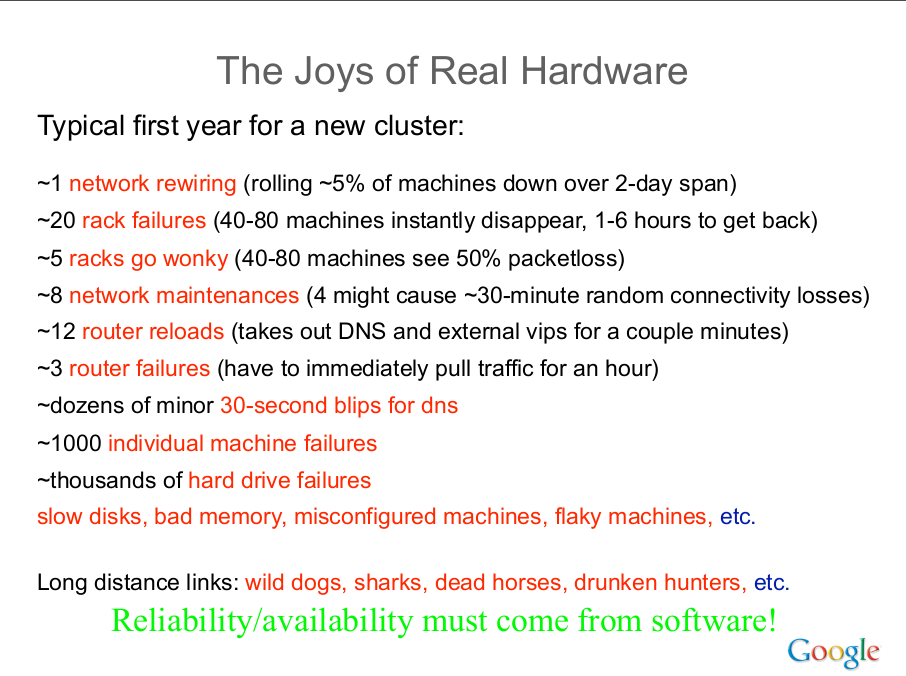
\includegraphics[scale=.45]{jeff_dean_hardware_wrong_google_2010_stanford.png}
\end{frame}


\begin{frame}{What Else Can Go Wrong? RAM}
\begin{itemize}
\item RAM bits flip
\begin{itemize}
	\item \underline{\textcolor{red}{\href{https://en.wikipedia.org/wiki/Soft_error\#Cosmic_rays_creating_energetic_neutrons_and_protons}{IBM}}}: cosmic rays can flip bits in RAM
	\item Server could crash, Data could get corrupted
	\item 256MB, one bit flip per month(in 1996)
	\item \underline{\textcolor{red}{\href{https://www.intelligentmemory.com/support/faq/ecc-dram/how-often-do-ecc-correctable-single-bit-errors-occur-and-how-about-double-multi-bit-errors.php}{Google}}}: one bit flip per 14 to 40 hours per Gigabyte of RAM, not evenly distributed though\note{some machines have alot, some don't have, age screw it, datacenter is good}
	\item Solution: ECC RAM\note{you can read somewhere on servers, 64 bit one error could be corrected}
\end{itemize}
\end{itemize}
\end{frame}



\begin{frame}{What Else Can Go Wrong? Disks}
	\begin{itemize}
		\item Storage \underline{\textcolor{red}{\href{https://en.wikipedia.org/wiki/Data_degradation\#In_storage}{bits flip on their own}}}
		\begin{itemize}
			\item SSD electric charges leaks away 
			\item HDD magnetic orientation change changes\note{specially in warm/humid area}
			\item Google back in 2005 \note{sorting 1TB of data, nearly sorted, pdf included in the repo}
			\item Today SSD/HDD have ECC inside
			\item URE \note{https://serverfault.com/a/79922/367171}
			\item Kingston: URE for consumer SSD 1 in 110TB read, Enterprise 1 in 1110TB read(Don't trust them with numbers)
			\item Some drives have way more often\note{likely production fault, One drive from 2017 have more than 2M faults)}
			\item Facebook RAID controller wrote data in the middle of the disks on boot(firmware problem)\note{facebook btrfs talk}
			\item Solution:
			\begin{itemize}
				\item RAID 5?
				\item RAID 1?
				\item BTRFS/ZFS/Ceph/... store hash, check it on every read, recover from specific implementation RAID.
			\end{itemize}
		\end{itemize}
	\end{itemize}
\end{frame}



\begin{frame}{Bit rot effect example}
	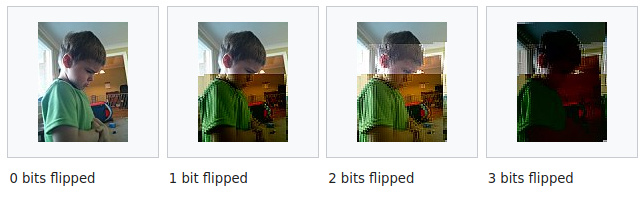
\includegraphics[scale=.7]{bitrot_example.png}
\end{frame}


\begin{frame}{What Can Go Wrong? the Human Factor}
	\begin{itemize}
		\item Wiped a production db myself :) \note{nimkat}
		\item Getting Hacked(like arvan)\note{other examples like aram}
		\item Getting Ransomwares
	\end{itemize}
\end{frame}


\begin{frame}
	\begin{center}
		\Huge Solutions
	\end{center}
\end{frame}

\begin{frame}{Backup Desiderata}
	\begin{itemize}
%		animate
		\item Take very little space
		\item Encrypted
		\begin{itemize}
			\item If Backup storage gets exposed means everything is in the open
		\end{itemize}
		\item Multiple versions of data
		\item Pruning versions By Grandfather-Father-Son
		\item Deduplicated, reduced space
	\end{itemize}
\end{frame}


\begin{frame}{Backup Desiderata: Not using Borg}
\begin{itemize}
	\item Disk failure shouldn't cause data loss
	\item Server failure shouldn't effect availability
	\item Disks bit-rot shouldn't affect the data
	\item Backup files getting exposed should make them accessible
	\item Malicious ones can't delete backups(even if the backup taker server gets exposed)
\end{itemize}
\end{frame}
\begin{frame}{My Solution}
\begin{itemize}
\item Borg + BTRFS RAID1 on at least two locations  

\item BTRFS RAID1 removes bit-rot problem

\item Two locations alleviates availability problems

\item Rsync.net and BTRFS snapshots solves immutability 
\end{itemize}
	 
\end{frame}

\begin{frame}{What is BorgBackup}
	BorgBackup (short: Borg) deduplicating backup program(compressed and encrypted authenticated)
\end{frame}

\begin{frame}{Borg Features}
	\begin{itemize}
	\item cli backup tool, separate GUIs

	\item good arch / platform / fs support

	\item deduplication 

	\item compression  

	\item auth. encryption\note{proves authenticity of data too}

	\item read from locally mounted fs

	\item store to local fs or to remote borg
	
	\item Fuse-mount backup archives

	\item HW-accelerated crypto
	\item Computational intensive stuff written in C, others in Python
	\item Uses single core(con)
\end{itemize}
\end{frame}

\begin{frame}{Borg as a Project}
	\begin{itemize}
		
	\item community project
	
	\item FOSS  (BSD license)
	
	\item Python 3.7(current, 3.6-9 supproted)
	
	\item for speed:  a little Cython \& C
	
	\item good docs  (for users, devs)
	
	\item good test coverage(83\% today), travis CI
	
	\item github: borgbackup/community
	\item Pays money for security bugs(~10,500\$ paid till 2020)  
\end{itemize}
\end{frame}
%https://camo.githubusercontent.com/9fc113ee23c824302ed977c516eb08b7d1b1e0db600b7186737bd32400f93976/68747470733a2f2f61736369696e656d612e6f72672f612f3133333239322e706e67

\begin{frame}{In Practice}
	\begin{itemize}
		\item size of postgres db 
		\item 48 hourly
		\item 20 daily 
		\item Weekly 6
		\item Monthly ...
		\item 78 instances  each ~2GB
		\item all:153.06 GB
		\item compressed 41.24 GB
		\item deduplicated 22.50 GB
	\end{itemize}
\end{frame}
\begin{frame}{In Practice}
\begin{itemize}
	\item media folder of a big django project 
	\item 3 instances each about 63 GB
	\item 182.70 GB compressed all instances(incompressible mostly already compressed images)
	\item 60.13 GB deduplicated across time
\end{itemize}
\end{frame}

\begin{frame}{In Practice}
	- a little changing postgres db 
	
	- 12 instances
	
	- 7 daily 
	
	- 4 weekly 
	
	- 1 monthly 
	
	- 2.75 GB all 
	
	- compressed 180MB
	
	- deduplicated 30 MB
\end{frame}

\begin{frame}{In Practice}
	- a wordpress site files  
	
	- 32 instances   
	
	- 80 GB total   
	
	- 70 GB compressed(incompressible mostly images)  
	
	- deduplicated 2.68 GB
	
\end{frame}

\begin{frame}{In Practice}
	- a wordpress site db
	
	- 32 instances
	
	- 5.5 GB
	
	- 420 MB compressed
	
	- 204 MB deduped
\end{frame}

\begin{frame}{In Practice}
	- a lot of mail boxes
	
	- 20 instances
	
	- 20 daily
	
	- total 727GB
	
	- 348 GB compressed(compressible since it is text)
	
	- deduped 17.5 GB
\end{frame}

\begin{frame}{In Practice}
	Total size: 1145 GB
	
	Fitted in ~103GB
\end{frame}

\begin{frame}{It scales well}
	one of developers of borg
	borg info ssh://borg@myserver/repos/myrepo
	
	Original size  22.76 TB
	
	 Compressed size 18.22 TB
	 
	   Dedup size 486.20 GB
	   
	Unique chunks 6305006
	
	         Total chunks                          272643223
\end{frame}

\begin{frame}{Where to put the data}
	
	Own a server with ssh and free space:
	
	install borg, configure, done!
	
	No remote server? No problem:
	\begin{itemize}
		\item rsync.net (ssh, cli)
		\item hetzner's storage box
		\item borgbase.com (ssh, web, easy)
		\item local repo + rclone to cloud
	\end{itemize}
\end{frame}

\begin{frame}{Deduplicating}
	dedup does \textbf{NOT} depend on:
	\begin{itemize}
		\item file/directory names: 
		\begin{itemize}
			\item move file even between machines, no change required
		\end{itemize}
		 \item Whole file hash and timestamps:
		 \begin{itemize} 
		 	\item only a small part of a file changed,only the change, VMs , or raw disks, only changes are synced.
		\end{itemize}
		
		\item Place of chunk in a file:
		\begin{itemize}
			\item stuff moved around inside a file , doesn't increase it.
		\end{itemize} 
	
	\end{itemize}
\end{frame}

%\begin{frame}{Speed}
%	speed:
%	
%	- perf-critical code in C/Cython(chunking, compression, encryption)
%	
%	- local caches file/chunks index data
%	
%	- quick detection of unmodified data
%	
%\end{frame}

\begin{frame}{Encryption}
	Enc :
	\begin{itemize}
		\item  Tampering/Corruption detection by HMAC or blake2b
		
		%	- note:(less cpu better than HMAC-SHA256)
		\item 256 bit AES- CTR
		
		\item uses OpenSSL(libcrypto)
		
		\item Passphrase and a key, could be separate
		
		\item PDKDF2 100K rounds
		
	\end{itemize}
\end{frame}

\begin{frame}{Compression}
	works on deduplicated block level
\begin{itemize}
	\item none
	\item lz4: fast, low compression(faster than no compression :-| )
	\item zstd: from high speed low compression to slow and high compression 
	\item zlib: medium speed and compression
	\item lzma: low speed, high compression
	\item auto: first lz4 it(superfast), if its  size have been reducedin size(compressible) then compress with other schemes.
\end{itemize}
\end{frame}

\begin{frame}{Safe} 
	borg uses:
	- checksums
	- transactions
	- fs: syncing, atomic ops
	- checkpoint while backing up
\end{frame}

\begin{frame}[fragile]
	\begin{lstlisting}[backgroundcolor = \color{black},
		basicstyle=\color{lightgray}
			language = bash,
			framexleftmargin = 1em]
# initialize a repository:
borg init /tmp/borg

# create a "first" archive inside this repo (verbose): 
borg create --progress --stats\

 /tmp/borg::first ~/Desktop


# create a "second" archive (less verbose):
borg create /tmp/borg::second ~/Desktop

# even more verbose:
borg create -v --stats /tmp/borg::third ~/Desktop
\end{lstlisting}
\end{frame}

\begin{frame}[fragile]
	\begin{lstlisting}[backgroundcolor = \color{black},
		basicstyle=\color{lightgray}
		language = bash,
		framexleftmargin = 1em]
# list repo / archive contents:

borg list /tmp/borg
borg list /tmp/borg::first

# extract ("restore") from an archive to cwd:

mkdir test ; cd test
borg extract /tmp/borg::third

# simulate extraction (good test):
borg extract -v --dry-run /tmp/borg::third

# check consistency of repo:
borg check /tmp/borg
\end{lstlisting}
\end{frame}



\begin{frame}[fragile]
	\begin{lstlisting}[backgroundcolor = \color{black},
		basicstyle=\color{lightgray}
		language = bash,
		framexleftmargin = 1em]
		# list repo / archive contents:
		
		borg list /tmp/borg
		borg list /tmp/borg::first
		
		# extract ("restore") from an archive to cwd:
		
		mkdir test ; cd test
		borg extract /tmp/borg::third
		
		# simulate extraction (good test):
		borg extract -v --dry-run /tmp/borg::third
		
		# check consistency of repo:
		borg check /tmp/borg
	\end{lstlisting}
\end{frame}
\note{
BTRFS; done
picture of bit rot from github; done
Borgmatic;  done
Healthcheck.io; done
No compression and auto; done 
fs snapshots for immutability; done
}
\begin{frame}{New Generation Filesystems}
\begin{itemize}
	\item Bit rot protection(check and fix on each read)
	\item It has fast space efficient snapshot \note{not like LVM}
	\item Use RAID1(RAID5/6 not stable)
	\item ZFS works, Ceph/S3 most other new things have this too.
	\item Run scrub periodically(reads all data and fix)
	\item Keep snapshots, and rotate them on your own(even if the client gets exposed, can't delete snapshots)
	\item openSUSE's default filesystem
	\item super efficient diff snapshot transfer to other locations
\end{itemize}
\end{frame}


\begin{frame}{Borgmatic}
	A tool for automation for backup with a lot of useful stuff
	\begin{itemize}
		\item Config is a YAML file
		\item Rotation Scheme is written in YAML
		\item Supports pre/post execution hooks
		\item Monitoring using healthchecks.io and others
	\end{itemize}
\end{frame}



\begin{frame}{Healthchecks.io}
	An opensource Scheduled-Job monitoring.
	
	Cron schedule are defined in the site, a token is given.

	Check start, end and non execution of job and alert properly
	
\end{frame}


\begin{frame}{rsync.net}
	Provide ssh accessible, backup space storage
	
	Has geo-redundant option too
	
	Minimum space is 400GB for 10\$/month(17.5\$/month for geo-redundant)
	
	ZFS with RAID is the underlaying file system
	
	7 free daily immutable snapshot.
	
	Configurable cron time for more immutable snapshots.
	
	 Extra ones is counted against your quota but ZFS snapshots are block levels diffs, thus it is only actually overwritten/added blocks of data not a new copy of it
\end{frame}


\begin{frame}{What we do for backups?}
	\begin{itemize}
		\item For new env, setup ssh access on backup client and storage server using ansible
		\item install proper borg version using ansible 
		\item install borgmatic using pip in the same ansible playbook
		\item Write a borgmatic YAML config(from templates available for different usecases across the company)
		\item Add proper cron schedule at healthchecks.io and add the token to YAML file
		\item put borgmatic in crontab
	\end{itemize}
\end{frame}
\begin{frame}{Faults}
	Trusting borg
	
	SSH to outside countries sometimes is problematic
	
	Populating a db from SQL dumps could be time consuming
	
	
\end{frame}

\end{document}
